\subsection{\rbt}\label{sec:Barney} % Section voor Barney


\Gls{RBV} came as a response to \gls{InBV} by~\cite{Porter:1980to} and was introduced by among others~\cite{Barney:1991ur,Wernerfelt:1984hx}
Nowadays more and more scholars are using the term \rbt.
\begin{quote}
  scholars are increasingly using the term resource-based theory instead of
resource-based view.
This reflects the fact that resource-based research has reached a level of
precision and sophistication such that it more closely resembles a theory than a 
view~\cite{Barney:2011jp}.
\end{quote}
This logic will be continued in this thesis.
Contrary to~\cite{Porter:1980to}, \rbt researched the link between firm's internal characteristics and it's performance~\cite{Barney:1991ur}.\\
Key in all this is that \rbt assumes that (a) firms across one industry may be heterogeneous with respect to strategic resources and (b) that resources are not perfectly mobile across firms hence heterogeneity may be long lasting~\cite{Barney:1991ur}.
%The key assumptions in \rbt (and thus \rbv) are that (a) firms within an industry may be heterogeneous with respect to the strategic resources they control and (b) these resources are may not be perfectly mobile across firms.
%This makes that the heterogeneity can be long lasting~\cite{Barney:1991ur}.
%\Gls{RBV} argues that a firms strategic advantage is depended on it's heterogeneous resources (a bundle of all assets, knowledge, and capabilities) which have to be the following:

The \acrlong{RBT} argues that firms posses resources, a subset of which enables them to achieve competitive advantage and a further subset which leads to superior long-term performance~\cite{Barney:1991ur,Wernerfelt:1984hx,Grant:1991wg}.
Studies of firm performance using \acrfull{RBV} have found differences not only between firms in similar industry but also within narrower groups within 
industries~\cite{Hansen:1989um,Cool:1988vw}.
The resources that are mentioned are defined as \textit{assets and capabilities that are available and useful in detecting and responding to market opportunities or threats}~\cite{sanchez:1996,Wade:2004wf}.
Where \textit{assets} are anything tangible or intangible the firm can use in it's processes for creating, producing and/or offering it's products (or services) to a 
market~\cite{sanchez:1996}.
And \textit{capabilities} are repeatable patterns of actions in the use of assets to create produce and/or offer products to a market~\cite{sanchez:1996}.

\begin{enumerate}[(a)]
   \setlength{\itemsep}{1pt}
\item must be valuable, in the sense that it exploit opportunities and/or neutralises threats in a firm’s environment
\item must be rare among a firm’s current and potential competition 
\item must be imperfectly imitable
\item  there cannot be strategically equivalent substitutes for this resource that are valuable but neither rare or imperfectly imitable 
\end{enumerate} 
The list of that is itemised is also known as the VRIN framework~\citep{Barney:1991ur}.
 

Later~\citep{Oliver:1997wj} added to the \rbt~by providing the following definition:
\begin{quote}
A resource-based view proposes that resource selection and accumulation are a function of both within-firm decision-making and external strategic factors~\citep{Oliver:1997wj}.
\end{quote}
This unique combination of resources will lead to~\ca~\cite{Barney:1991ur}. \\
\rbt is not without it's critiques~\citep{Narayanan:2005wy,Kraaijenbrink:2009bu,Priem:2001vd,Dung:2012wh}.
Some more detail on the critiques on~\cite{Barney:1991ur} can be found in Appendix~\ref{app:critiques_barney}.\\
In his paper 2011 paper~\cite{Barney:2011jp} concludes that \rbt~and therefore also \rbv~is not on the decline.
The fact that \rbt~is still in use in recently published papers perhaps speaks more volume on the fact that the theory can still be considered relevant~\citep{Mukherjee:2013vz,Hoskisson:2012jk,Lockett:2013jr}.

\begin{figure}[htbp] 
	\centering
	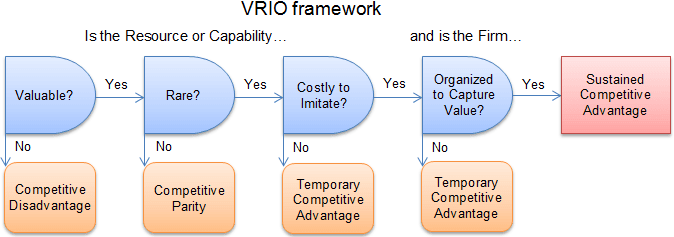
\includegraphics[width=0.8\textwidth]{vrio_framework}
 	\caption[The VRIO framework]{The VRIO framework. Adapted from~\citep{rothaermel2012strategic}}\label{fig:VRIO}
\end{figure}


The VRIN framework developed in~\cite{Barney:1991ur} was also extended and improved upon~\cite{Barney:1995tz} just as he had improved on the terminology of \rbt.
\cite{Barney:1995tz} introduced the concept of VRIO\@.
\begin{description} 
   \setlength{\itemsep}{1pt}
\item[The Question of Value] Resources are valuable if they help organisations to increase the value offered to the customers. This is done by increasing differentiation or/and decreasing the costs of the production. The resources that cannot meet this condition, lead to competitive disadvantage.

\item[The Question of Rarity] Resources that can only be acquired by one or few companies are considered rare. When more than few companies have the same resource or capability, it results in competitive parity.

\item[The Question of Imitability] A company that has valuable and rare resource can achieve at least temporary competitive advantage. However, the resource must also be costly to imitate or to substitute for a rival, if a company wants to achieve sustained competitive advantage.

\item[The Question of Organisation] The resources itself do not confer any advantage for a company if it’s not organised to capture the value from them. Only the firm that is capable to exploit the valuable, rare and imitable resources can achieve sustained competitive advantage\footnote{adopted from~\citep{Strategic-management-insight:2013}}.
\end{description}

The key improvement to the VRIO (see also~\ref{fig:VRIO}) framework from the VRIN framework is the addition of the question if the organisation is ready and capable to exploit all the resources~\citep{Barney:1995tz,Strategic-management-insight:2013}.
The point is that all this should again lead to~\ca through~\glspl{FSA}~\citep{Barney:1991ur,Barney:2001tj,Barney:2011jp}. 
The frameworks by~\citep{Barney:1991ur,Barney:1995tz} lead to the following:

\begin{WP}\label{wp:rbt}
  The diversity in internal resources (humans and knowledge) within firms could be responsible for the heterogeneity of firms responses to changes institutional environment
\end{WP}

\subsection{Firm specific resources}

A key concept of~\cite{Barney:1991ur,Barney:2001tj} is that the different (internal) resources lead to~\glspl{FSA}.
The resources of MNE are by definition located in the host and home country of that MNE\@. 
\cite{Barney:1991ur,Barney:1995tz} suggests that ``resources within the firm are not perfectly mobile across firms and that heterogeneity can be long lasting''~\citep{Barney:1991ur}.
Whether this assumption holds true is a matter of discussion.
The fact that resources might be (perfectly) mobile given certain constraints has been brought up~\citep{Lavie:2006up,Priem:2001vd} already.\\
\cite{Hu:1995vg} identified that the firm's advantages are indeed transferable, be it with varying amounts of success (certain constraints).
The success are visible through the expansion of Hong Kong firms in East Asia~\citep{Hu:1995vg}.
However these similar firms expanding to the US or Great Britain yielded a different story~\citep{Hu:1995vg}.\\
The same holds for (high-tech) Korean firms expanding to \glsfull{EE} and \glsfull{AE}. 
Here a difference strategies was observed while sill dealing with comparable MNEs~\citep{Erramilli:1997wu}.
The same firm specific resources were employed in different capacities relative to the market that was entered.\\
Not only the economic regions that are entered are relevant to the methods and impact resources have on the MNE\@.
The type of resource has a profound effect on its capacity to be either internationally mobile or immobile~\citep{Tseng:2007wm}.\\
Some \fsa have in the form of resources have different characteristics in general. 
\cite{Rugman:2001ti} differentiates between three types of resources.
\begin{enumerate}[(a)]
   \setlength{\itemsep}{1pt}
\item Non location bound \fsa
\item Location bound \fsa 
\item Subsidiary specific advantages
\end{enumerate}
Where the (non) location bound \fsa are in it self to be exploited globally and easy to diffuse locally (a) or hard to exploit globally and provide local national responsiveness (b) the subsidiary specific advantages are a different animal by itself. 
They are easy to deploy globally but difficult to exploit internally~\citep{Rugman:2001ti}.
The subsidiary specific advantages display characteristics of perfectly mobile resources as they are very mobile across firms, but not within firms or MNEs.\\
The observations above relax the statement of~\cite{Barney:1991ur} somewhat as to the perfect mobility of resources.
According to~\citep{Rugman:2001ti,Tseng:2007wm,Erramilli:1997wu,Hu:1995vg,Rugman:1992uj} some consideration has to be given to the fact that resources are perfectly immobile according to \rbt.
This may not be always a certainly.
This depends off course on a case by case basis as indicated above.
 
%The theory of Barney is \emph{introspective}. 
%It takes into account what is happening inside the firm.
%What knowledge is available, the people matter. 
%Processes that have been created over time are a contributing factor. 
%In the 1970's Toyota engineered \gls{tpm} for it's factories this gave them \gls{CA} over their US rivals as production cost were lower for their products.
%Only if these resources cannot be imitated in an other country and location this can create a \gls{CA}.
%In contrast to~\gls{RBV} the theory of~\cite{Porter:1980to} is thus~\emph{extrospective} and does not consider the company itself.\\
%Actually both theories are not mutually exclusive. They are very well capable of existing simultaneously. 
%This line of thought give rise to the fact that there might be a third pillar in strategy thinking.